\documentclass[a4paper,12pt]{article}
\usepackage[T2A]{fontenc}
\usepackage[utf8]{inputenc}
\usepackage[russian]{babel}
\usepackage{amsmath}
\usepackage{graphicx}
\usepackage{array}
\usepackage{multirow}
\usepackage{setspace}
\usepackage{float}
\usepackage{hyperref}
\usepackage{indentfirst}
\usepackage[left=3cm,right=1.5cm,top=2cm,bottom=2cm]{geometry}

\newcommand{\ministry}{МИНИСТЕРСТВО НАУКИ И ВЫСШЕГО ОБРАЗОВАНИЯ РОССИЙСКОЙ ФЕДЕРАЦИИ}
\newcommand{\university}{Федеральное государственное бюджетное образовательное учреждение высшего образования}
\newcommand{\universityname}{АДЫГЕЙСКИЙ ГОСУДАРСТВЕННЫЙ УНИВЕРСИТЕТ}
\newcommand{\faculty}{Инженерно-физический факультет}
\newcommand{\department}{Кафедра автоматизированных систем обработки информации и управления}
\newcommand{\reporttitle}{Отчёт по практике}
\newcommand{\reporttheme}{Решение системы линейных алгебраических уравнений методом Гаусса}
\newcommand{\studentinfo}{2 курс, группа 2ИВТ}
\newcommand{\studentname}{Л. Д. Котенков}
\newcommand{\supervisor}{С. В. Теплоухов}
\newcommand{\cityyear}{Майкоп, 2025 г.}

\begin{document}

% Титульный лист
\begin{titlepage}
    \vspace*{0.5cm}
    \centering
    
    \textbf{\ministry}
    
    \vspace{0.3cm}
    \university
    
    \vspace{0.3cm}
    \textbf{\universityname}
    
    \vspace{0.5cm}
    \faculty
    
    \department
    
    \vspace{2cm}
    \textbf{\reporttitle}
    
    \vspace{0.5cm}
    \textbf{\reporttheme}
    
    \vspace{2cm}
    \studentinfo
    
    \vfill
    
    \begin{flushright}
        \begin{minipage}{7cm}
            \noindent
            Выполнил: \\
            \underline{\hspace{3.8cm}} \studentname \\
            «\underline{\hspace{0.7cm}}» \underline{\hspace{2.5cm}} 2025 г. \\
            
            \vspace{0.5cm}
            
            Руководитель: \\
            \underline{\hspace{3.8cm}} \supervisor \\
            «\underline{\hspace{0.7cm}}» \underline{\hspace{2.5cm}} 2025 г. \\
        \end{minipage}
    \end{flushright}
    
    \vspace{1cm}
    \cityyear
\end{titlepage}

% Оглавление
\newpage
\renewcommand{\contentsname}{Оглавление}
\tableofcontents

\newpage
\section{Теория}
Метод Гаусса --- классический метод решения системы линейных алгебраических уравнений (СЛАУ). Это метод последовательного исключения переменных, когда с помощью элементарных преобразований система уравнений приводится к равносильной системе треугольного вида, из которой последовательно, начиная с последних (по номеру), находятся все переменные системы.

\textbf{Алгоритм решения СЛАУ методом Гаусса подразделяется на два этапа.}

На первом этапе осуществляется так называемый прямой ход, когда путём элементарных преобразований над строками систему приводят к ступенчатой или треугольной форме, либо устанавливают, что система несовместна. А именно, среди элементов первого столбца матрицы выбирают ненулевой, перемещают его на крайнее верхнее положение перестановкой строк и вычитают получившуюся после перестановки первую строку из остальных строк, домножив её на величину, равную отношению первого элемента каждой из этих строк к первому элементу первой строки, обнуляя тем самым столбец под ним. После того, как указанные преобразования были совершены, первую строку и первый столбец мысленно вычёркивают и продолжают пока не останется матрица нулевого размера. Если на какой-то из итераций среди элементов первого столбца не нашёлся ненулевой, то переходят к следующему столбцу и проделывают аналогичную операцию.

На втором этапе осуществляется так называемый обратный ход, суть которого заключается в том, чтобы выразить все получившиеся базисные переменные через небазисные и построить фундаментальную систему решений, либо, если все переменные являются базисными, то выразить в численном виде единственное решение системы линейных уравнений. Эта процедура начинается с последнего уравнения, из которого выражают соответствующую базисную переменную (а она там всего одна) и подставляют в предыдущие уравнения, и так далее, поднимаясь по «ступенькам» наверх. Каждой строчке соответствует ровно одна базисная переменная, поэтому на каждом шаге, кроме последнего (самого верхнего), ситуация в точности повторяет случай последней строки.

В простейшем случае алгоритм выглядит так:

\begin{figure}[H]
\centering
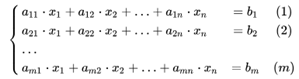
\includegraphics[width=0.7\textwidth]{image1.png}
\caption{Прямой ход метода Гаусса}
\end{figure}

Прямой ход:

\begin{figure}[H]
\centering
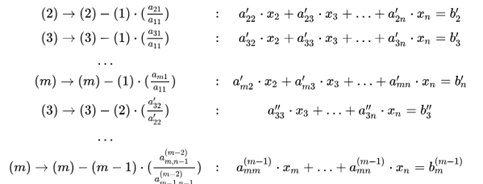
\includegraphics[width=0.7\textwidth]{image2.png}
\caption{Детализация прямого хода}
\end{figure}

Обратный ход. Из последнего ненулевого уравнения выражаем базисную переменную через небазисные и подставляем в предыдущие уравнения. Повторяя эту процедуру для всех базисных переменных, получаем фундаментальное решение.

\section{Код программы}
\begin{verbatim}
#include <iostream>
#include <cmath>
using namespace std;

const double EPS = 1e-9;
const int MAX_SIZE = 10;

void printSystem(double matrix[MAX_SIZE][MAX_SIZE + 1], int n) {
    for (int i = 0; i < n; i++) {
        for (int j = 0; j < n; j++) {
            cout << matrix[i][j] << " ";
        }
        cout << "| " << matrix[i][n] << endl;
    }
    cout << endl;
}

int main() {
    setlocale(0, "ru");
    int n;
    double matrix[MAX_SIZE][MAX_SIZE + 1] = { 0 };
    
    while (true) {
        cout << "Введите количество уравнений (1-" << MAX_SIZE << "): ";
        cin >> n;
        if (cin.good() && n > 0 && n <= MAX_SIZE) break;
        cout << "Ошибка! Введите число от 1 до " << MAX_SIZE << endl;
        cin.clear();
        cin.ignore(10000, '\n');
    }
    
    cout << "Введите коэффициенты системы (по строкам):\n";
    for (int i = 0; i < n; i++) {
        for (int j = 0; j <= n; j++) {
            while (true) {
                cin >> matrix[i][j];
                if (cin.good()) break;
                cout << "Ошибка! Введите число: ";
                cin.clear();
                cin.ignore(10000, '\n');
            }
        }
    }
    
    cout << "\nИсходная система:\n";
    printSystem(matrix, n);
    
    for (int col = 0; col < n; col++) {
        int max_row = col;
        for (int i = col + 1; i < n; i++) {
            if (abs(matrix[i][col]) > abs(matrix[max_row][col])) {
                max_row = i;
            }
        }
        
        if (max_row != col) {
            swap(matrix[col], matrix[max_row]);
            cout << "Меняем строки " << col + 1 << " и " << max_row + 1 << ":\n";
            printSystem(matrix, n);
        }
        
        if (abs(matrix[col][col]) < EPS) {
            cout << "Система вырождена!\n";
        }
        
        for (int j = n; j >= col; j--) {
            matrix[col][j] /= matrix[col][col];
        }
        
        cout << "Нормализуем строку " << col + 1 << ":\n";
        printSystem(matrix, n);
        
        for (int i = col + 1; i < n; i++) {
            double factor = matrix[i][col];
            for (int j = col; j <= n; j++) {
                matrix[i][j] -= factor * matrix[col][j];
            }
            cout << "Обнуляем строку " << i + 1 << ":\n";
            printSystem(matrix, n);
        }
    }
    
    for (int i = 0; i < n; i++) {
        bool all_zero = true;
        for (int j = 0; j < n; j++) {
            if (abs(matrix[i][j]) > EPS) {
                all_zero = false;
                break;
            }
        }
        if (all_zero && abs(matrix[i][n]) > EPS) {
            cout << "Нет решений!\n";
        }
    }
    
    double solution[MAX_SIZE] = { 0 };
    for (int i = n - 1; i >= 0; i--) {
        solution[i] = matrix[i][n];
        for (int j = i + 1; j < n; j++) {
            solution[i] -= matrix[i][j] * solution[j];
        }
    }
    
    cout << "Решение системы:\n";
    for (int i = 0; i < n; i++) {
        cout << "x" << i + 1 << " = " << solution[i] << endl;
    }
}
\end{verbatim}

\section{Пример работы программы}
\begin{figure}[H]
\centering
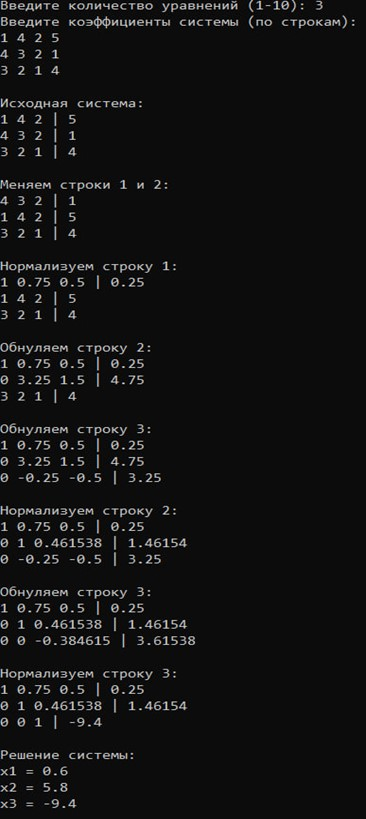
\includegraphics[width=0.5\textwidth]{image3.jpeg}
\caption{Пример работы программы}
\end{figure}

\end{document}